% siminos/spatiotemp/Examples/examSymm1d.tex
% $Author: predrag $ $Date: 2021-08-25 23:18:52 -0400 (Wed, 25 Aug 2021) $

\renewcommand{\Refl}{\ensuremath{{\sigma}}} % conflict with ``symmetric''

%%%%%%%%%%%%%%%%%%%%%%%%%%%%%%%%%%%%%%%%%%%%%%%%%%%%%%%%%%%%%%%
\FIG{
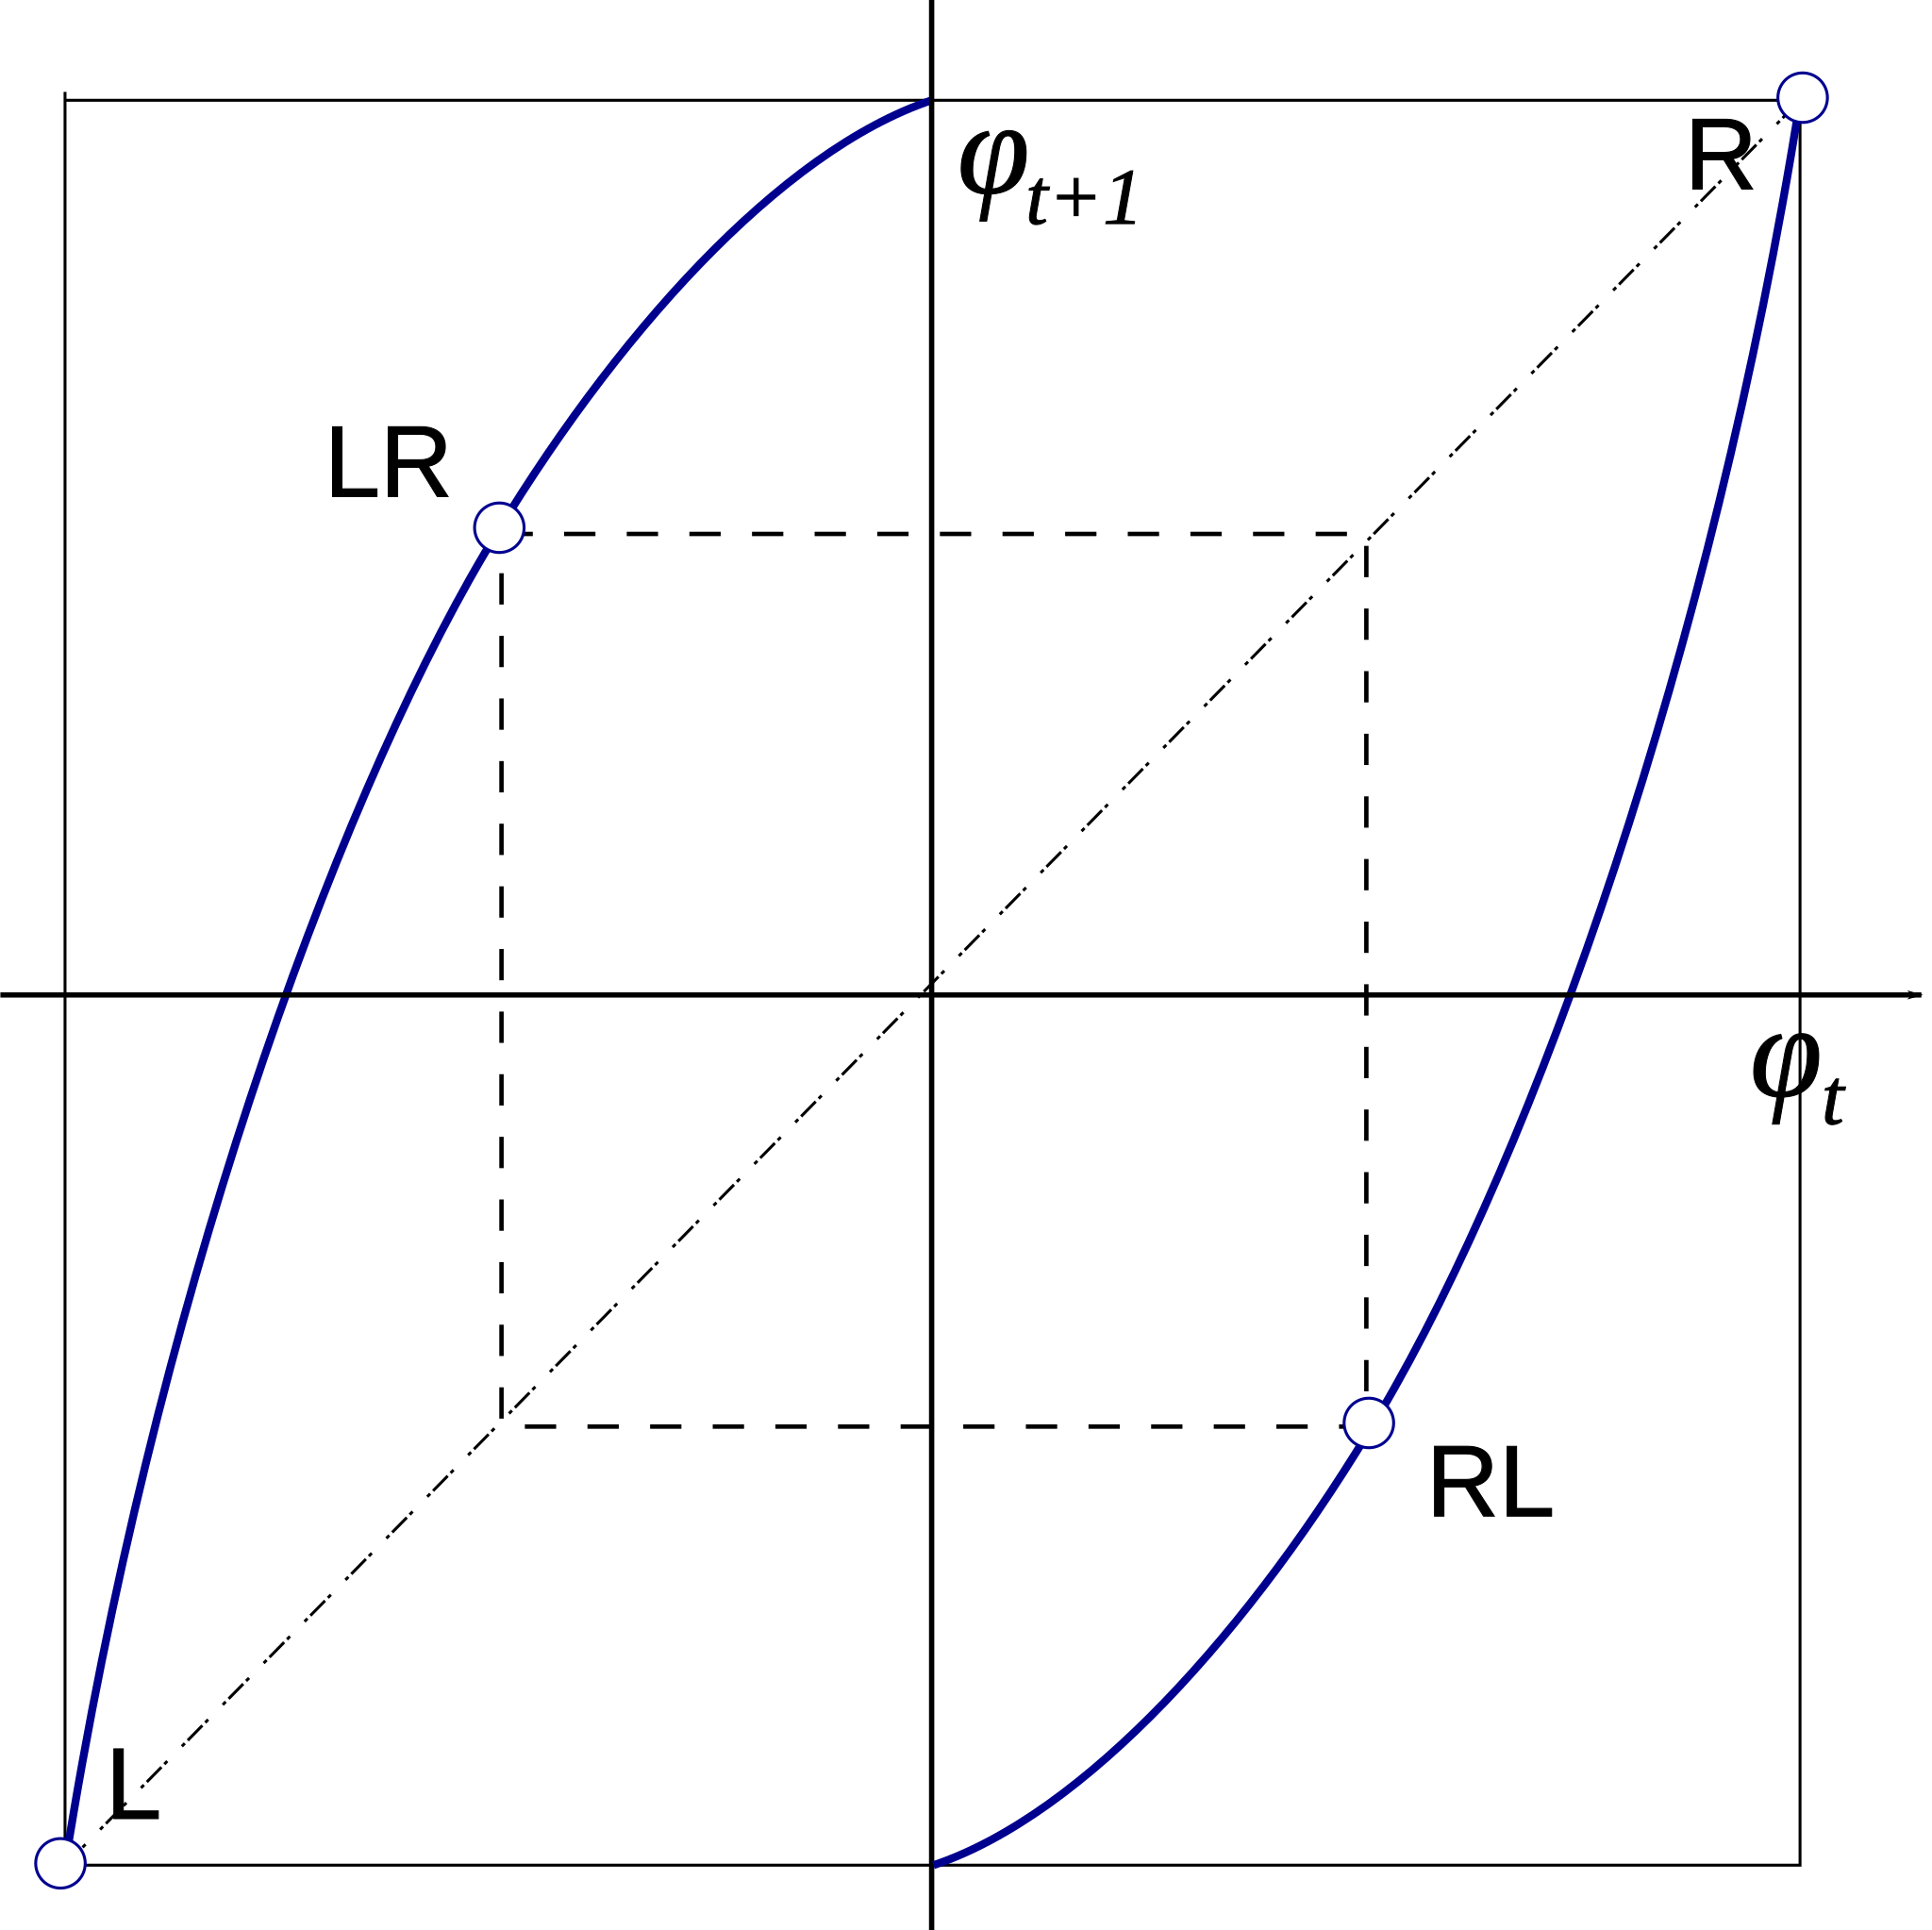
\includegraphics[width=0.35\textwidth]{BernBent}
}{}{
The $\Dn{1}$-equivariant `bent Bernoulli' map has two types of
\po s:
(a)
asymmetric pairs, such as the fixed points pair $\{\cycle{L},\cycle{R}\}$.
(b) $\Dn{1}$-symmetric ({setwise} invariant) \po s, such as the 2-cycle \cycle{LR},
composed of the relative cycle segment from $L$ to $R$
and its repeat from $R$ to $L$.
~~(study \refexam{exam:Symm1d};
   continued in \reffig{Symm1d:BernBentFund})
}{Symm1d:BernBent}
%%%%%%%%%%%%%%%%%%%%%%%%%%%%%%%%%%%%%%%%%%%%%%%%%%%%%%%%%%%%%%%

%%%%%%%%%%%%%%%%%%%%%%%%%%%%%%%%%%%%%%%%%%%%%%%%%%%%%%%%%%%%%%%%%%
\FIG{
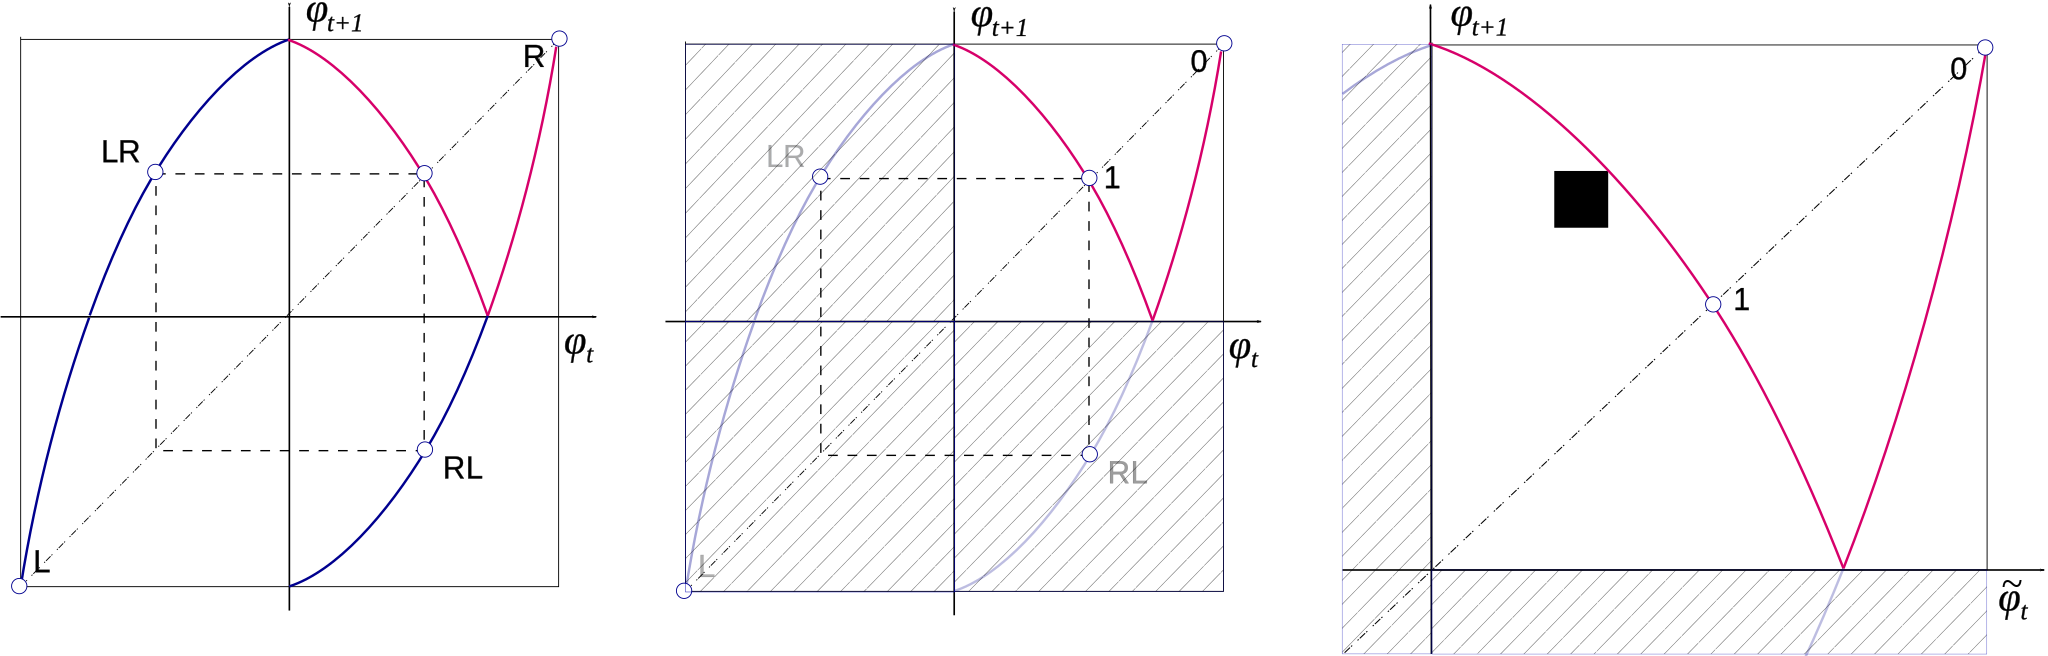
\includegraphics[width=0.80\textwidth]{BernBentFund}
}{}{
The `bent Bernoulli' map of \reffig{Symm1d:BernBent}
with the $\Dn{1}$ symmetry $f(-\field)=-f(\field)$, restricted to the
fundamental domain. $f(\field)$ is indicated by a blue line, and
fundamental domain map ${\tilde\map}({\tilde \field})$ by the purple line.
The asymmetric fixed point pair \{\cycle{L},\cycle{R}\} is reduced to the
fixed point \cycle{0}, and the full \statesp\ symmetric 2-cycle
\cycle{LR} is reduced to the fixed point \cycle{1}.
~~(work through \refexam{exam:Symm1d})
% continued in #\reffig{??}).
}{Symm1d:BernBentFund}
%%%%%%%%%%%%%%%%%%%%%%%%%%%%%%%%%%%%%%%%%%%%%%%%%%%%%%%%%%%%%%%

%%%%%%%%%%%%%%%%%%%%%%%%%%%%%%%%%%%%%%%%%%%%%%%%%%%%%%%%%%%%%%%
% from \2020-12-18 Chapter{smale}{16jan2014}{Stretch, fold, prune}
%Table 4
\begin{table}
\caption[]{\small Correspondence between the $\Dn{1}$ symmetry
reduced cycles $\tilde{p}$ and the full \statesp\
periodic orbits ${p}$, together with their
multiplicities $m_p$. Also listed are the two shortest cycles
(length 6) related by time reversal, but distinct under $\Dn{1}$.
}
{\small
\begin{tabular}{lll}
%\hline
$\tilde{p}$ & ${p}$  & $m_p$ \\
\hline
 0  & $R$ & 2 \\
 1 & $LR$ & 1 \\ %\hline
 01 & $LLRR$   & 1 \\ %\hline
 011 & $LLR$  & 2 \\
 001 & $LLLRRR$ & 1 \\
%\hline
 0111 & $LRLLRLRR$  & 1 \\
 0001 & $LRRR$ & 2 \\
 0011 & $LLLLRRRR$ & 1 \\
%\hline
 01111 & $LRLRL$ & 2 \\
 00111 & $LRLLLRLRRR$  & $1$ \\
 11010 & $LRRLLRLLRR$ & $1$ \\
 00011 & $LRLLLRLRRR$   &    $1$ \\
 10100 & $LLRRR$   &    $2$ \\
 00001 & $LLLLLRRRRR$ & $1$ \\
%\hline
 110100 & $LRRLLLRLLRRR$ & $1$ \\
 110010 & $LRRRLLRLLLRR$ & $1$ %\\
%\hline
\end{tabular}
} %end \small
\label{dscr:t-symm-4}
\end{table}
%%%%%%%%%%%%%%%%%%%%%%%%%%%%%%%%%%%%%%%%%%%%%%%%%%%%%%%%%%%%%%%

%%%%%%%%%%%%%%%%%%%%%%%%%%%%%%%%%%%%%%%%%%%%%%%%%%%%%%%%%%%%%%%%%%%%%%%
\example{\Dn{1}-reduced binary symbolic dynamics.}{  \label{exam:Symm1d}
% was \section{$\Zn{2} = \Dn{1}$ factorization}
% was \label{s-C-2-fact} in ChaosBook - REPLACE!
% was section siminos/spatiotemp/chapter/symm1d.tex
% Predrag                               20sep2017
% extracted from symm.tex {Discrete symmetry factorization}
% Predrag                                7apr2015
\index{dihedral group!\Dn{1}}
\index{group!\Dn{1}}                                    \toCB

    \PC{2017-09-20}{
Extracted this %\refsect{s-C-2-fact}
from ChaosBook \texttt{symm.tex} {\em Discrete symmetry factorization},
\toChaosBook{section.25.5}
{sect.~25.5} {\em $\Zn{2} = \Dn{1}$ factorization}
(version of 2015-04-07).
    }
%    \PC{2021-08-01}{
% Drew a bent Bernoulli map; like Bernoulli, but the two branches are curved}
%
Consider a nonlinear, $\Dn{1}$-symmetric `bent Bernoulli' map  of
\reffig{Symm1d:BernBent}; like the bimodal map \reffig{dscr:f_1d_symm_a},
but with the middle interval squeezed to a point, so the symbolic
dynamics is simpler, complete binary with  a 2-letter alphabet $L$(eft),
$R$(ight).

In \reffig{Symm1d:BernBentFund} the fundamental domain map
${\tilde\map}({\tilde\field})$ is obtained by reflecting $\field < 0$
segments of the global map $f(\field)$ into the upper right quadrant.
${\tilde\map}$ also has two branches, with $\tilde{\pS} = [0,1]$ split
into two regions $\tilde{\pS} = \{\tilde{\pS}_0,\tilde{\pS}_1\}$ which we
label with a 2-letter alphabet $\tilde{\alphabet} = \{0,1\}$. While the
full \statesp\ map has two monotone branches with positive slopes, the
symmetry reduced map is a unimodal map, with negative slope branch
$\tilde\map_1$.

The negative slope branch is the consequence of relative periodicity: the
mirror image of the $\ssp_\sym$ periodic point is reached by traversing
the \rpo\ segment $\symf$  of length $\nsymf$, $\flow{\nsymf}{\ssp_\sym}
= \Refl \ssp_\sym $, see the $LR$ 2-cycle in \reffig{Symm1d:BernBent}, so
the \rpo\ temporal {\JacobianM} carries a minus sign.

We could have illustrated this with the Bernoulli piecewise linear map,
\reffig{fig:BernPart}, whose symmetry-reduced map is the Ulam tent map,
but there the \Dn{1} symmetry is so obvious that it is hidden in the
plain sight.
       \PC{2021-08-03}{
Make up the Bernoulli \Dn{1}-symmetry example, setting up
\refexam{exam:BernD1zeta}, will need it for \textbf{LC21}.
        }

The symbolic dynamics is again complete binary dynamics, with any
sequence of letters $\{0,1\}$ \admissible.
Assume that all \po s are strictly unstable, $|\ExpaEig_p>0|$,  so that
each orbit or orbit is uniquely labeled by an infinite string
$\{\Ssym{i}\}$, $\Ssym{i}\in\{R,L\}$, and that the dynamics is invariant
under the $ R \leftrightarrow L $ interchange, \ie, it is $\Dn{1}$
symmetric. The \po s separate into the symmetric orbits
\(
\sym\in\{RL, RRLL, RRRLLL, RLLRLRRL, \cdots\}
\,,
\)
with multiplicity $m_\sym=1$, and the asymmetric orbit pairs
\(
\asym\in\{R, L, RRL, LLR, \cdots\}
\,,
\)
with multiplicity $m_\asym=2$. For example, as there is no
distinction between % the ``up" and the ``down" spins, or
the ``left" or the ``right" branch of the map, the weights
$t_R=t_L$,  $t_{RRL}=t_{RLL}$, are equal, and so on.
\exerbox{e_Lor_Ising}

The symmetry reduced labeling $\symf_i \in \{0,1\}$ is related to the full
\statesp\ labels $\Ssym{i} \in \{L,R\}$ % L(eft), R(ight) % was Ising spin
by
\bea
\mbox{If} \quad \Ssym{i} & = & \Ssym{i-1} \quad \mbox{then} \quad \symf_i=0
     \continue
\mbox{If} \quad \Ssym{i} & \neq & \Ssym{i-1} \quad \mbox{then} \quad \symf_i=1
\eea
For example, both $\cycle{L}=\cdots{LLLL}\cdots$ and
$\cycle{R}=\cdots{RRRR}\cdots$ map into $\cdots{000}\cdots=\cycle{0}$,
$\cycle{LR}=\cdots{LRLR}\cdots$ maps into $\cdots{111}\cdots=\cycle{1}$,
$\cycle{LRRL}=\cdots{LLRRLLRR}\cdots$
maps into $\cdots{0101}\cdots = \cycle{01}$, and so forth.
A list of such reductions is given in  \reftab{dscr:t-symm-4}.
   \PC{2021-08-02}{
    please recheck \reftab{dscr:t-symm-4}: I have interchanged `0' and
    `1' compared to ChaosBook, might have introduced errors.}
%
~~(continued in \refexam{exam:Fact1d},
   illustrated by the Bernoulli \refexam{exam:BernD1zeta})
\index{Ising model}
                                        \jumpBack{exam:Symm1d}
    } %end \example{exam:Symm1d}
%%%%%%%%%%%%%%%%%%%%%%%%%%%%%%%%%%%%%%%%%%%%%%%%%%%%%%%%%%%%%%%%%%%%%%%

\renewcommand{\Refl}{\ensuremath{{s}}} % Dihedral wiki convention
